\documentclass[12pt, titlepage]{article}

\usepackage{graphicx}
\usepackage{float}
\usepackage{booktabs}
\usepackage{tabularx}
\usepackage{hyperref}
\hypersetup{
    colorlinks,
    citecolor=black,
    filecolor=black,
    linkcolor=red,
    urlcolor=blue
}
\usepackage[round]{natbib}

%% Comments

\usepackage{color}

\newif\ifcomments\commentstrue %displays comments
%\newif\ifcomments\commentsfalse %so that comments do not display

\ifcomments
\newcommand{\authornote}[3]{\textcolor{#1}{[#3 ---#2]}}
\newcommand{\todo}[1]{\textcolor{red}{[TODO: #1]}}
\else
\newcommand{\authornote}[3]{}
\newcommand{\todo}[1]{}
\fi

\newcommand{\wss}[1]{\authornote{blue}{SS}{#1}} 
\newcommand{\plt}[1]{\authornote{magenta}{TPLT}{#1}} %For explanation of the template
\newcommand{\an}[1]{\authornote{cyan}{Author}{#1}}

%% Common Parts

\newcommand{\progname}{Mechtronics Enigeering} % PUT YOUR PROGRAM NAME HERE
\newcommand{\authname}{Team 32, Wingman
\\ Edward He
\\ Erping Zhang
\\ Guangwei Tang
\\ Peng Cui
\\ Peihua Jin } % AUTHOR NAMES                  

\usepackage{hyperref}
    \hypersetup{colorlinks=true, linkcolor=blue, citecolor=blue, filecolor=blue,
                urlcolor=blue, unicode=false}
    \urlstyle{same}
                                


\begin{document}

\title{Verification and Validation Report: \progname} 
\author{\authname}
\date{\today}
	
\maketitle

\pagenumbering{roman}

\section{Revision History}

\begin{tabularx}{\textwidth}{p{3cm}p{2cm}X}
\toprule {\bf Date} & {\bf Version} & {\bf Notes}\\
\midrule
2023/3/7 & 1.0 & Finish the required parts\\
2023/3/8 & 1.1 & Fix errors\\
\bottomrule
\end{tabularx}

~\newpage


\section{Purpose}
This document is intended to support the systematic plan for testing the functionality of the system. It meant to show the system has met the requirements in both software and hardware aspects mentioned in requirements document. In particular, this document will describe the testing results. By the end of testing process, it can be shown that the system is working properly and available for usage.
\section{Scope}
The document would pay attention to the different functionalities being discussed within the VnVPlan documentation. In addition, it would undergo the testing processes as if it was a black box, which will emphasis on the inputs and outputs of the system instead of the internal process and mechanics.	
\section{Background}	
SmartVault is designed to assist the user to remember where his/her belongings are and the most recent time the user had used or placed their belongings. The proposed system is capable of tracking and following human activities to position itself best for capturing any moving objects caused by the user. The system will identify each item that is being moved and record/update their corresponding positions. The user then has the ability to interact with our system through an interface and select which item the user is looking for. Given this information, our system would identify where that specific item is and assist the user to locate their belongings in a short time.
This section will not be appropriate for every project.
~\newpage
\section{Functional Requirements Evaluation}

\subsubsection{Area of Testing1}
		
\paragraph{Manual Testing}{Testing shown:}
\begin{table}[H]
\begin{center}
\begin{tabular}{|l | m{9cm}|}
\hline
  Test Number & IPR1-1\\
  \hline
  Requirement Reference & IPR1\\
  \hline
  Requirement &  The system should be able to identify human’s body\\
  \hline
  Input & Images of the working environment and a human show up in
the environment\\
  \hline
  Desired Output & Coordinate of the detected human body\\
  \hline
  Actual Output & Correct coordinate of the detected human body\\
  \hline
  Conclusion & The test pass as expected\\
  \hline
\end{tabular}
\end{center}           
\end{table}


\begin{table}[H]
\begin{center}
\begin{tabular}{|l | m{9cm}|}
\hline
  Test Number & IPR3-1\\
  \hline
  Requirement Reference & IPR3\\
  \hline
  Requirement &  The system should be able to identify new objects introduced in the area\\
  \hline
  Input & Images of the working environment with new objects in the environment\\
  \hline
  Desired Output & Coordinate of the detected new objects and outlining them with boxes\\
  \hline
  Actual Output & Correct Coordinate of the detected new objects and outlining them with boxes\\
  \hline
  Conclusion & The test pass as expected\\
  \hline
\end{tabular}
\end{center}           
\end{table}

\begin{table}[H]
\begin{center}
\begin{tabular}{|l | m{9cm}|}
\hline
  Test Number & IPR4-1\\
  \hline
  Requirement Reference & IPR4\\
  \hline
  Requirement &  The system should be able to identify moving objects in the area\\
  \hline
  Input & Images of the working environment with object in different location in the environment\\
  \hline
  Desired Output & Coordinate of the new location of detected moving objects and highlight the new location\\
  \hline
  Actual Output & Correct Coordinate of the new location of detected moving objects and highlight the new location\\
  \hline
  Conclusion & The test pass as expected\\
  \hline
\end{tabular}
\end{center}           
\end{table}




\begin{table}[H]
\begin{center}
\begin{tabular}{|l | m{9cm}|}
\hline
  Test Number & IPR4-1\\
  \hline
  Requirement Reference & IPR4\\
  \hline
  Requirement &  To create 3 folders sequentially\\
  \hline
  Input & createFolder() being called\\
  \hline
  Desired Output & 3 folders (FolderScreenShot, item, location) created\\
  \hline
  Actual Output & 3 folders (FolderScreenShot, item, location) created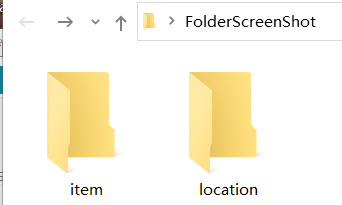
\includegraphics[width=80mm, height=55mm]{UT1.png}\\
  \hline
  Conclusion & Pass\\
  \hline
\end{tabular}
\end{center}           
\end{table}
\begin{table}[H]
\begin{center}
\begin{tabular}{|l | m{9cm}|}
\hline
  Test Number & IPR4-2\\
  \hline
  Requirement Reference & IPR4\\
  \hline
  Requirement &  Do nothing if they have already existed\\
  \hline
  Input & createFolder() being called\\
  \hline
  Desired Output & No change\\
  \hline
  Actual Output & No change\\
  \hline
  Conclusion & Pass\\
  \hline
\end{tabular}
\end{center}           
\end{table}
\begin{table}[H]
\begin{center}
\begin{tabular}{|l | m{9cm}|}
\hline
  Test Number & IPR5-1\\
  \hline
  Requirement Reference & IPR5\\
  \hline
  Requirement &  To store the initial frame\\
  \hline
  Input & (1, 'i')\\
  \hline
  Desired Output & Adding item1\_\{date and time\}.png,  item1.png\\
  \hline
  Actual Output & Added as:\\&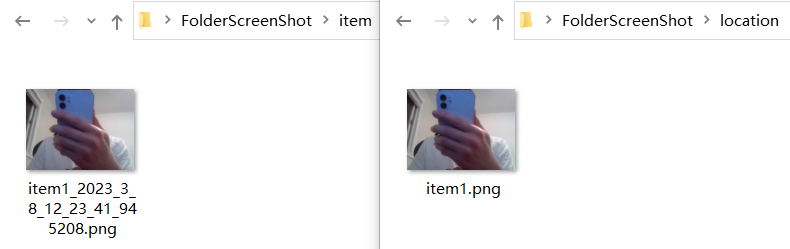
\includegraphics[width=90mm, height=35mm]{UT2.png}\\
  \hline
  Conclusion & Pass\\
  \hline
\end{tabular}
\end{center}           
\end{table}
\begin{table}[H]
\begin{center}
\begin{tabular}{|l | m{9cm}|}
\hline
  Test Number & IPR5-2\\
  \hline
  Requirement Reference & IPR5\\
  \hline
  Requirement &  To check whether the frame is stored in the correct path\\
  \hline
  Input & (1, 'i')\\
  \hline
  Desired Output &  item\{num\}\_\{date and time\}.png is stored in 'item', item\{num\}.png is stored in 'location'\\
  \hline
  Actual Output &  item1\_2023\_3\_8\_12\_23\_41\_945208.png is within 'item', item1.png is inside 'location'\\&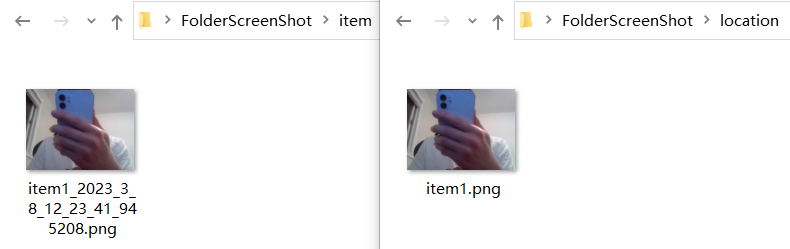
\includegraphics[width=90mm, height=35mm]{UT2.png}\\
  \hline
  Conclusion & Pass\\
  \hline
\end{tabular}
\end{center}           
\end{table}
~\newpage
\paragraph{Automatic Testing}{Testing shown:}
\begin{table}[H]
\begin{center}
\begin{tabular}{|l | m{9cm}|}
\hline
  Test Number & IPR6-1\\
  \hline
  Requirement Reference & IPR5, IPR6\\
  \hline
  Requirement & To check whether the frame for the second item is captured\\
  \hline
  Input & (2, 'i')\\
  \hline
  Desired Output & Adding item2\_\{date and time\}.png, item2.png\\
  \hline
  Actual Output & Added as:\\&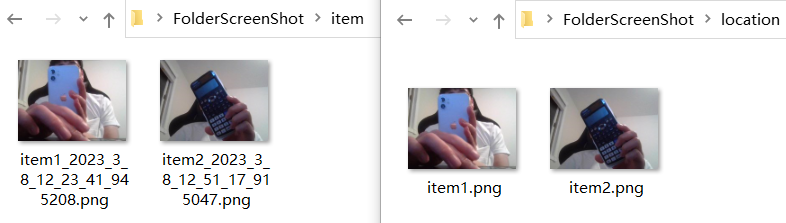
\includegraphics[width=90mm, height=33mm]{UT3.png}\\
  \hline
  Conclusion & pass\\
  \hline
\end{tabular}
\end{center}           
\end{table}
\begin{table}[H]
\begin{center}
\begin{tabular}{|l | m{9cm}|}
\hline
  Test Number & IPR6-2\\
  \hline
  Requirement Reference & IPR4, IPR6\\
  \hline
  Requirement &  To check whether the location frame for the first item is updated, meanwhile the second item won't get affected\\
  \hline
  Input & (1, 'u')\\
  \hline
  Desired Output & item1\_\{date and time\}.png should remain, item1.png shall be updated\\
  \hline
  Actual Output & Only item1.png get updated\\&Comparison shown:\\&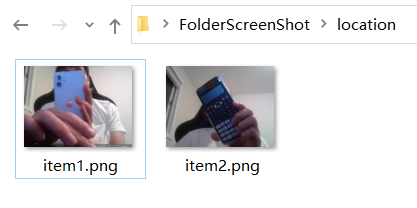
\includegraphics[width=90mm, height=46mm]{UT41.png}\\&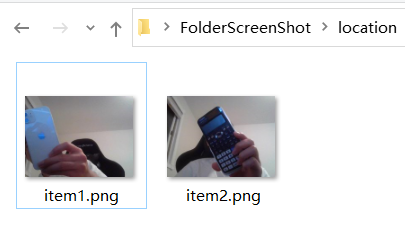
\includegraphics[width=89mm, height=48mm]{UT42.png}\\
  \hline
  Conclusion & Pass\\
  \hline
\end{tabular}
\end{center}           
\end{table}
\subsubsection{UI Interface Menu}
\paragraph{Manual Testing}{Testing shown:}
\begin{table}[H]
\begin{center}
\begin{tabular}{|l | m{9cm}|}
\hline
  Test Number & UIR1-1\\
  \hline
  Requirement Reference & UIR1\\
  \hline
  Requirement & The UI should notify the user when the user has a wrong password input \\
  \hline
  Input & The wrong input of the password\\
  \hline
  Desired Output & There should be a text notification shown on the window\\
  \hline
  Actual Output & 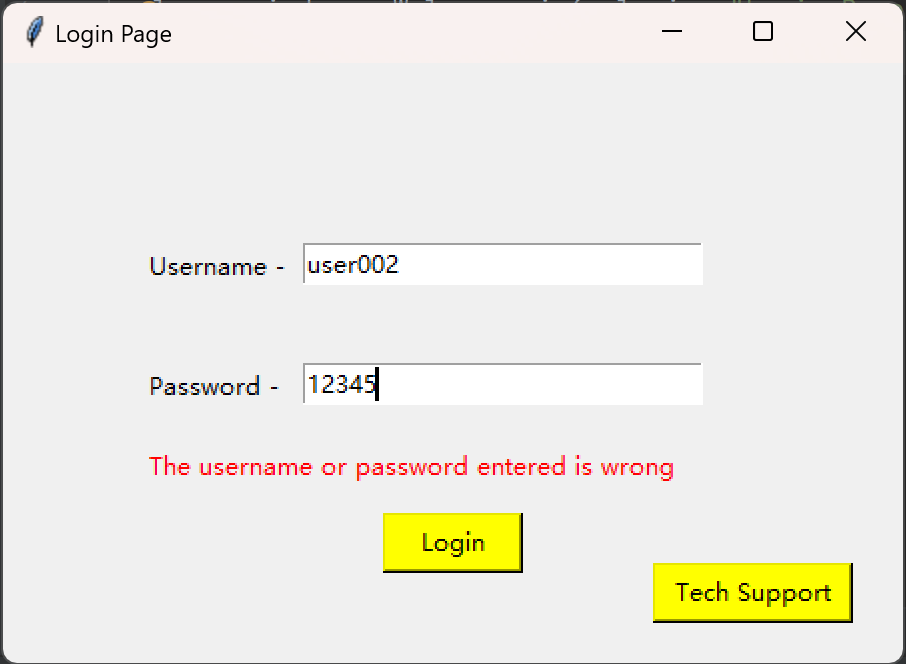
\includegraphics[width=80mm, height=55mm]{UIR11.png}\\
  \hline
  Conclusion & The test is successful\\
  \hline
\end{tabular}
\end{center}           
\end{table}

\begin{table}[H]
\begin{center}
\begin{tabular}{|l | m{9cm}|}
\hline
  Test Number & UIR1-2\\
  \hline
  Requirement Reference & UIR1\\
  \hline
  Requirement & The UI should notify the user when the user has a wrong username input \\
  \hline
  Input & The wrong input of the username\\
  \hline
  Desired Output & There should be a text notification shown on the window\\
  \hline
  Actual Output & 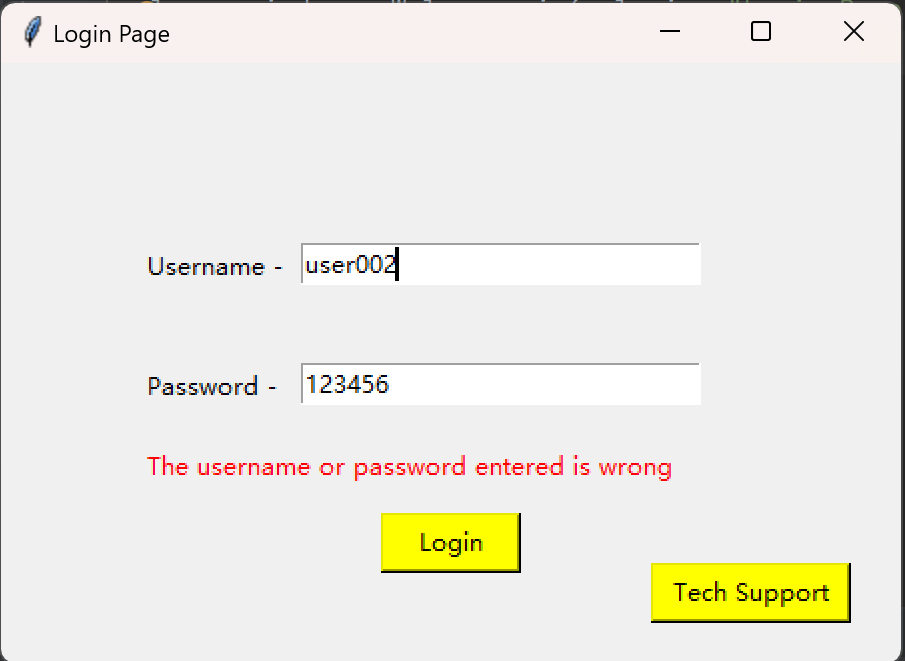
\includegraphics[width=80mm, height=55mm]{UIR12.png}\\
  \hline
  Conclusion & The test is successful\\
  \hline
\end{tabular}
\end{center}           
\end{table}

\begin{table}[H]
\begin{center}
\begin{tabular}{|l | m{9cm}|}
\hline
  Test Number & UIR2-1\\
  \hline
  Requirement Reference & UIR2\\
  \hline
  Requirement & The UI should be able to let the user to switch the pictures shown in the window \\
  \hline
  Input & The next button is clicked\\
  \hline
  Desired Output & A different picture is shown\\
  \hline
  Actual Output & A different picture is shown in the window\\
  \hline
  Conclusion & The test is successful\\
  \hline
\end{tabular}
\end{center}           
\end{table}

\begin{table}[H]
\begin{center}
\begin{tabular}{|l | m{9cm}|}
\hline
  Test Number & UIR2-2\\
  \hline
  Requirement Reference & UIR2\\
  \hline
  Requirement & The UI should be able to let the user to switch the pictures shown in the window \\
  \hline
  Input & The previous button is clicked\\
  \hline
  Desired Output & A different picture is shown\\
  \hline
  Actual Output & A different picture is shown in the window \\
  \hline
  Conclusion & The test is successful\\
  \hline
\end{tabular}
\end{center}           
\end{table}

\begin{table}[H]
\begin{center}
\begin{tabular}{|l | m{9cm}|}
\hline
  Test Number & UIR3-1\\
  \hline
  Requirement Reference & UIR3\\
  \hline
  Requirement & The UI should be able to provide information about the location of the item \\
  \hline
  Input & The user select the item picture\\
  \hline
  Desired Output & The location of the picture is shown in a new window\\
  \hline
  Actual Output & \\
  \hline
  Conclusion & The test is successful\\
  \hline
\end{tabular}
\end{center}           
\end{table}

\begin{table}[H]
\begin{center}
\begin{tabular}{|l | m{9cm}|}
\hline
  Test Number & UIR3-2\\
  \hline
  Requirement Reference & UIR3\\
  \hline
  Requirement & The UI should be able to provide information about the location of the item \\
  \hline
  Input & The user select the item picture\\
  \hline
  Desired Output & The UI should notify the user that the item has been taken out of the room\\
  \hline
  Actual Output & \\
  \hline
  Conclusion & The test is successful\\
  \hline
\end{tabular}
\end{center}           
\end{table}


\begin{table}[H]
\begin{center}
\begin{tabular}{|l | m{9cm}|}
\hline
  Test Number & UIR4-1\\
  \hline
  Requirement Reference & UIR4\\
  \hline
  Requirement & The UI should be able to let the user to choose the information input\\
  \hline
  Input & The user select the choose box\\
  \hline
  Desired Output & The UI provides choices to the user\\
  \hline
  Actual Output & 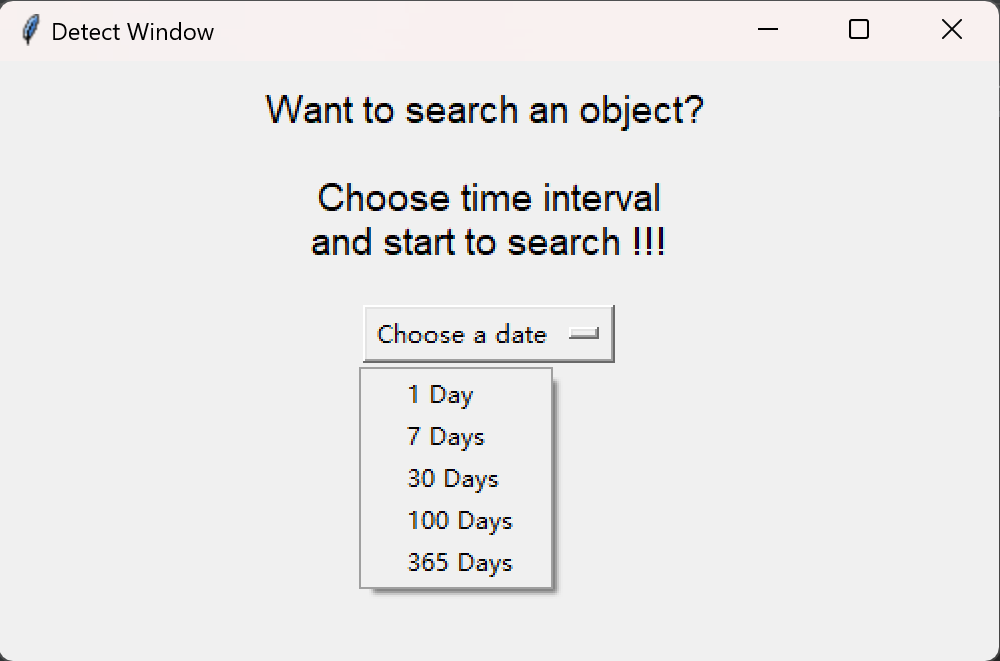
\includegraphics[width=80mm, height=55mm]{UIR41.png}\\
  \hline
  Conclusion & The test is successful\\
  \hline
\end{tabular}
\end{center}           
\end{table}

\section{Nonfunctional Requirements Evaluation}

\subsection{Usability and Humanity Requirements}

\begin{table}[H]
\begin{center}
\begin{tabular}{|l | m{9cm}|}
\hline
  Test Number & APR1-1\\
  \hline
  Requirement Reference & APR1\\
  \hline
  Requirement & The User is able to launch the program without help\\
  \hline
  Input & The servy paper\\
  \hline
  Desired Output & An average of high rating shown on the paper\\
  \hline
  Actual Output &\\
  \hline
  Conclusion & The test is successful\\
  \hline
\end{tabular}
\end{center}           
\end{table}

\begin{table}[H]
\begin{center}
\begin{tabular}{|l | m{9cm}|}
\hline
  Test Number & EUR1-1\\
  \hline
  Requirement Reference & EUR1\\
  \hline
  Requirement & The User is able to use the hardware without help\\
  \hline
  Input & The servy paper\\
  \hline
  Desired Output & An average of high rating shown on the paper\\
  \hline
  Actual Output &\\
  \hline
  Conclusion & The test is successful\\
  \hline
\end{tabular}
\end{center}           
\end{table}

\begin{table}[H]
\begin{center}
\begin{tabular}{|l | m{9cm}|}
\hline
  Test Number & EUR2-1\\
  \hline
  Requirement Reference & EUR2\\
  \hline
  Requirement & The User is able to find the desired item without help\\
  \hline
  Input & The servy paper\\
  \hline
  Desired Output & An average of high rating shown on the paper\\
  \hline
  Actual Output &\\
  \hline
  Conclusion & The test is successful\\
  \hline
\end{tabular}
\end{center}           
\end{table}

\begin{table}[H]
\begin{center}
\begin{tabular}{|l | m{9cm}|}
\hline
  Test Number & LER1-1\\
  \hline
  Requirement Reference & LER1\\
  \hline
  Requirement & The User is able to install the software without help\\
  \hline
  Input & The servy paper\\
  \hline
  Desired Output & An average of high rating shown on the paper\\
  \hline
  Actual Output &\\
  \hline
  Conclusion & The test is successful\\
  \hline
\end{tabular}
\end{center}           
\end{table}

\begin{table}[H]
\begin{center}
\begin{tabular}{|l | m{9cm}|}
\hline
  Test Number & LER2-1\\
  \hline
  Requirement Reference & LER2\\
  \hline
  Requirement & The program can take pictures after the user has been leave the room\\
  \hline
  Input & The user leave the room\\
  \hline
  Desired Output & Pictures are taken\\
  \hline
  Actual Output &\\
  \hline
  Conclusion & The test is successful\\
  \hline
\end{tabular}
\end{center}           
\end{table}

\begin{table}[H]
\begin{center}
\begin{tabular}{|l | m{9cm}|}
\hline
  Test Number & UPR1-1\\
  \hline
  Requirement Reference & UPR1\\
  \hline
  Requirement & The user is able to see each picture clearly\\
  \hline
  Input & The servy paper\\
  \hline
  Desired Output & An average of high rating shown on the paper\\
  \hline
  Actual Output &\\
  \hline
  Conclusion & The test is successful\\
  \hline
\end{tabular}
\end{center}           
\end{table}

\begin{table}[H]
\begin{center}
\begin{tabular}{|l | m{9cm}|}
\hline
  Test Number &  APR1-1 \\
  \hline
  Requirement Reference & ARP1 \\
  \hline
  Requirement & No electronic components should be visible and exposed. The mount should stay still without any physical changes  \\
  \hline
  Input & Launch the program normally and give the camera mount a physical impact \\
  \hline
  Desired Output & The mount should not be broken and there should not be any visible dislocation of any parts\\
  \hline
  Actual Output & The mount undergoes a planar movement. No visible parts broken or dislocation. The arduino board attached at the bottom stays still  \\
  \hline
  Conclusion & The test is successful\\
  \hline
\end{tabular}
\end{center}           
\end{table}

\begin{table}[H]
\begin{center}
\begin{tabular}{|l | m{9cm}|}
\hline
  Test Number & EUR1-1\\
  \hline
  Requirement Reference & EUR1\\
  \hline
  Requirement &  Users without electronics and coding background will be able to connect the hardware and use the program\\
  \hline
  Input & Users are asked to connect the hardware and start the program\\
  \hline
  Desired Output & There should not be any unclear instructions for the user to proceed. The hardware system including the Arduino board, camera and mount should be clarified for people to plug the wires\\
  \hline
  Actual Output & As camera,Arduino board and the motor are already attached to the mount. User just need to plug the wires to corresponding pins then they can simply start the program with one click \\
  \hline
  Conclusion & The test is successful\\
  \hline
\end{tabular}
\end{center}           
\end{table}

\begin{table}[H]
\begin{center}
\begin{tabular}{|l | m{9cm}|}
\hline
  Test Number & SCR3-1\\
  \hline
  Requirement Reference & SCR3\\
  \hline
  Requirement &  Rotation speed of the camera should be appropriate and will not damage other parts under the condition the camera have to rotate from one end to the other\\
  \hline
  Input & Human walk through the camera and leave the capture region at high pace\\
  \hline
  Desired Output & The camera will detect the human body and starts to follow the human movement. Once the human accelerate and leave the region, the camera will stop tracking and the rotation speed will not be fast enough to damage other parts\\
  \hline
  Actual Output & The camera will rotate to the human position and follow the movement once it detects the existence of human body. As the human quickly leave the capture region, the camera stops tracking and take a photo of the current frame. After 2 seconds, it will rotate back to the original position. There are no parts being damaged during the movement \\
  \hline
  Conclusion & The test pass as expected\\
  \hline
\end{tabular}
\end{center}           
\end{table}
\section{Changes Due to Testing}
	
\section{Traceability Matrices}
\subsection{Traceability for Functional Requirements}
\begin{tabular}{|p{0.33\textwidth}|p{0.33\textwidth}|p{0.33\textwidth}|}

\hline \multicolumn{3}{|c|}{Table 1: Traceability for Area of Testing 1}\\

\hline Test Method&Requirement&Test Number\\

\hline Manual&IPR1&IPR1-1\\

\hline Manual&IPR4&IPR4-1\\

\hline Manual&IPR4&IPR4-2\\

\hline Manual&IPR5&IPR5-1\\

\hline Manual&IPR5&IPR5-2\\

\hline Automatic&IPR5, IPR6&IPR6-1\\

\hline Automatic&IPR4, IPR6&IPR6-2\\

\hline

\end{tabular}
\\
\begin{tabular}{|p{0.33\textwidth}|p{0.33\textwidth}|p{0.33\textwidth}|}

\hline \multicolumn{3}{|c|}{Table 2: Traceability for UI Interface Menu}\\

\hline Test Method&Requirement&Test Number\\

\hline Manual&UIR1&UIR1-1\\

\hline Manual&UIR1&UIR1-2\\

\hline Manual&UIR2&UIR2-1\\

\hline Manual&UIR2&UIR2-2\\

\hline Manual&UIR3&UIR3-1\\

\hline Manual&UIR3&UIR3-2\\

\hline Manual&UIR4&UIR4-1\\

\hline

\end{tabular}
\subsection{Traceability for Nonfunctional Requirements}

\begin{tabular}{|p{0.33\textwidth}|p{0.33\textwidth}|p{0.33\textwidth}|}

\hline \multicolumn{3}{|c|}{Table 3: Traceability for Usability and Humanity Requirements}\\

\hline Test Method&Requirement&Test Number\\

\hline Manual&APR1&APR1-1\\

\hline Manual&EUR1&EUR1-1\\

\hline Manual&EUR2&EUR2-1\\

\hline Manual&LER1&LER1-1\\

\hline Manual&LER2&LER2-1\\

\hline Manual&UPR1&UPR1-1\\

\hline Manual&UIR4&UIR4-1\\

\hline Manual&SCR3&SCR3-1\\

\hline

\end{tabular}

\bibliographystyle{plainnat}
\bibliography{../../refs/References}

\newpage{}
\section*{Appendix --- Reflection}

The information in this section will be used to evaluate the team members on the
graduate attribute of Lifelong Learning.  Please answer the following questions:

\begin{enumerate}
  \item 
  \item 
\end{enumerate}

\end{document}
